\ProvidesFile{ch2.tex}[]

\chapter{Variational Bayesian Fluorescence Nanoscopy}
\ix{physics//Physics appendix}

\section{Background}

\subsection{The Bayesian calculation}
Bayesian inference provides a rigorous framework for updating beliefs about the world in light of new data. It leverages the principles of probability theory to combine prior knowledge with empirical evidence, resulting in updated, posterior beliefs. In parametric modeling, we assume that the data $x$ are generated from a distribution with a set of parameters $y$. Parametric models simplify the problem by assuming a specific form for the underlying distribution of the data, characterized by a finite set of parameters. This approach allows us to use mathematical functions to describe complex systems and make inferences about the parameters based on observed data.

At the heart of Bayesian inference is Bayes' rule, which allows us to update our beliefs based on new evidence. Bayes' rule is derived from the definition of conditional probability. For events $A$ and $B$, the conditional probability of $A$ given $B$ is defined as
\begin{equation*}
P(A \lvert B) = \frac{P(A \cap B)}{P(B)},
\end{equation*}
provided that $P(B) > 0$. Similarly, the conditional probability of $B$ given $A$ is
\begin{equation*}
P(B \lvert A) = \frac{P(A \cap B)}{P(A)}.
\end{equation*}
Rearranging these equations and solving for $P(A \cap B)$ gives us Bayes' rule:
\begin{equation*}
P(A \lvert B) = \frac{P(B \lvert A) P(A)}{P(B)}.
\end{equation*}

In Bayesian inference, we reinterpret these events in terms of data and parameters. Let $x$ denote the observed data and $y$ denote the parameters or latent variables of the model. Bayes' rule then becomes
\begin{equation*}
p(y \lvert x) = \frac{p(x \lvert y) p(y)}{p(x)}.
\end{equation*}
Here, $p(y \lvert x)$ is the posterior distribution, representing our updated beliefs about the parameters after observing the data. $p(x \lvert y)$ is the likelihood, the probability of the observed data given the parameters. $p(y)$ is the prior distribution, representing our beliefs about the parameters before observing the data. $p(x)$ is the marginal likelihood or evidence, which normalizes the posterior distribution and ensures it sums to one.

One of the main challenges in Bayesian inference is the computation of the posterior distribution. The denominator in Bayes' rule, $p(x)$, involves an integral over all possible values of the parameters:
\begin{equation*}
p(x) = \int p(x \lvert y) p(y) \, dy.
\end{equation*}
In many practical applications, this integral is intractable due to the high dimensionality of the parameter space. This intractability is often referred to as the curse of dimensionality, where the complexity of computations increases exponentially with the number of dimensions.

To address this challenge, various approximation methods have been developed. One such method is Markov Chain Monte Carlo (MCMC), which generates samples from the posterior distribution by constructing a Markov chain that has the desired distribution as its equilibrium distribution. MCMC methods, such as the Metropolis-Hastings algorithm and the Gibbs sampler, allow us to approximate the posterior distribution even when the exact integral is computationally infeasible.

MCMC algorithms were originally developed in the 1940s by physicists at Los Alamos. These physicists, including Ulam (inspired by playing solitaire!) and Von Neumann (who developed the acceptance-rejection algorithm), were interested in modeling the probabilistic behavior of atomic particles. They could not do this analytically, but they wondered if they could use simulation. Simulation was difficult as the normalization constant was not known. Moreover, simulation as a computational tool hadn't been widely adopted yet, although ideas around simulation had been around for some time – e.g., Buffon's needle (1700s), Lord Kelvin (1901), and Fermi (1930s). In fact, the term “Monte Carlo” was coined at Los Alamos.

Ulam and Metropolis overcame this problem by constructing a Markov chain for which the desired distribution was the stationary distribution of the Markov chain. They then only needed to simulate the Markov chain until stationarity was achieved. Towards this end, they introduced the Metropolis algorithm, and its impact was enormous. Afterwards, MCMC was introduced to statistics and generalized with the Metropolis algorithm and its variants as well as the Gibbs sampler \parencite{Geman1984}

Another approach to approximating the posterior distribution is variational inference. This method involves approximating the true posterior distribution $p(y \lvert x)$ with a simpler, parameterized distribution $q(y)$ by minimizing the Kullback-Leibler (KL) divergence between them. The KL divergence,
\begin{equation*}
D_{KL}(q(y) \lvert p(y \lvert x)),
\end{equation*}
measures how one probability distribution diverges from a second, expected probability distribution.

To minimize the KL divergence, we first express it as
\begin{equation*}
D_{KL}(q(y) \lvert p(y \lvert x)) = \int q(y) \log \frac{q(y)}{p(y \lvert x)} \, dy.
\end{equation*}
This can be rewritten using Bayes' rule as
\begin{equation*}
D_{KL}(q(y) \lvert p(y \lvert x)) = \int q(y) \log \frac{q(y) p(x)}{p(x \lvert y) p(y)} \, dy = \log p(x) + \int q(y) \log \frac{q(y)}{p(x \lvert y) p(y)} \, dy.
\end{equation*}
Since $\log p(x)$ is constant with respect to $q(y)$, minimizing $D_{KL}(q(y) \lvert p(y \lvert x))$ is equivalent to maximizing the Evidence Lower Bound (ELBO), defined as
\begin{equation*}
ELBO = \int q(y) \log \frac{p(x \lvert y) p(y)}{q(y)} \, dy.
\end{equation*}
Maximizing the ELBO ensures that $q(y)$ is as close as possible to the true posterior $p(y \lvert x)$. This approach provides a practical way to perform Bayesian inference, especially in high-dimensional settings where traditional methods may be computationally prohibitive.

In variational inference, model parameters and latent variables can be treated interchangeably. This flexibility allows us to use powerful optimization techniques to approximate complex posterior distributions and make Bayesian inference feasible for a wide range of applications.

\subsection{The curse of dimensionality}

Dimensionality refers to the number of variables or features in a dataset. In fluorescence nanoscopy, each spatial coordinate (e.g., x, y, and potentially z in three-dimensional imaging) and additional attributes such as time points or different fluorophore states contribute to the dimensionality of the data. As the number of these features increases, the dataset becomes high-dimensional. The curse of dimensionality is a term coined to describe various phenomena that arise when working with high-dimensional data, making statistical analysis and machine learning more challenging. Mathematically, the curse of dimensionality can be described through the following issues:

As dimensionality increases, the volume of the space grows exponentially. For instance, the volume of a hypercube with side length $l$ in $d$-dimensional space is given by $l^d$. This rapid increase in volume means that data points become sparser, making it difficult to estimate densities and find meaningful patterns. Furthermore, in high-dimensional spaces, the concept of distance becomes less informative. For example, the difference between the minimum and maximum distance between data points tends to shrink as dimensionality increases, which can make clustering and nearest-neighbor algorithms less effective. With a large number of dimensions, models can easily become overly complex, capturing noise instead of the underlying signal. This leads to overfitting, where the model performs well on training data but poorly on unseen data. High-dimensional data requires more computational resources for processing and storage. Algorithms that are efficient in low dimensions may become impractical in high dimensions due to increased time and space complexity.

\subsection{The Hierarchical Variational Autoencoder}

Variational Autoencoders (VAEs), introduced by Kingma and Welling in 2013, are a sophisticated class of generative models that combine principles of variational inference with deep learning. They provide a powerful framework for learning complex, high-dimensional data distributions by mapping data to a lower-dimensional latent space and then reconstructing the data from these latent representations.

To understand VAEs, it's essential to first appreciate their roots in Bayesian inference. Bayesian inference aims to update the probability estimate for a hypothesis as more evidence or information becomes available. The fundamental tool for this process is Bayes' theorem, which is expressed as:
\begin{equation*}
p(y \lvert x) = \frac{p(x \lvert y) p(y)}{p(x)}.
\end{equation*}
Here, $p(y \lvert x)$ is the posterior distribution of the latent variables $y$ given the data $x$, $p(x \lvert y)$ is the likelihood of the data given the latent variables, $p(y)$ is the prior distribution of the


\section{Abstract}

Fast extraction of physically relevant information from images using deep neural networks has led to significant advances in fluorescence microscopy and its application to the study of biological systems. For example, the application of deep networks for kernel density (KD) estimation in single molecule localization microscopy (SMLM) has accelerated super-resolution imaging of densely-labeled structures in the cell. However, simple and interpretable uncertainty quantification is lacking in these applications, and remains a necessary modeling component in high-risk research. We propose a generative modeling framework for KD estimation in SMLM based on variational diffusion. This approach allows us to probe the structure of the posterior on KD estimates, creating an additional avenue toward quality control. We demonstrate that data augmentation with traditional SMLM architectures followed by a diffusion process permits simultaneous high-fidelity super-resolution with uncertainty estimation of regressed KDEs. 

\section{Introduction}

Deep models have attracted tremendous attention from researchers in the natural sciences, with several foundational applications arising in microscopy \parencite{Weigert2018,Falk2019}. Recently, the application of deep image translation in single-molecule localization microscopy (SMLM) has received considerable interest. SMLM techniques are a mainstay of fluorescence microscopy, which localize ``blinking'' fluorescent molecules to produce a pointillist representation of biomolecules in the cell at diffraction-unlimited precision \parencite{Rust2006,Betzig2006}. Recently, the use of deep models to perform localization has been proposed as an alternative to traditional localization algorithms, in order to increase imaging speed and labeling density. In previous applications of deep models to localization microscopy, super-resolution images have been recovered from a sparse set of localizations with conditional generative adversarial networks \parencite{Ouyang2018} or localization itself can be performed using traditional convolutional networks \parencite{Nehme2020,Speiser2021}. In this paper, we perform localization indirectly by predicting kernel density (KD) estimates of a population of fluorescent molecules using a deep model. 

Kernel density estimation in SMLM is necessarily performed using a single low-resolution image, and thus common measures of model performance are based on localization errors computed over ensembles of simulated images. Unfortunately, this choice precludes computation of uncertainty at test time under a fixed model. Bayesian probability theory is therefore an attractive alternative, which offers us mathematically grounded tools to reason about uncertainty. 

We model a posterior on high-resolution KD estimates conditioned on a low-resolution image. Our approach is based on a type of score based generative model \parencite{Song2021}, referred to as a denoising diffusion probabilistic model (DDPM) in the literature \parencite{Ho2020,Song2021}. We find that this technique is complementary to relevant existing approaches to uncertainty estimation, which would primarily address epistemic sources of uncertainty, using techniques such as ensembling \parencite{Lakshminarayanan2017} or Monte Carlo dropout \parencite{Gal2022}. The approach is inspired by recent variational perspectives on diffusion \parencite{Dirmeier2023,Ribeiro2024,Kingma2021,Kingma2023}.  Such techniques provide a mechanism for scalable variational inference, which can be trained using a variational bound written in terms of the signal-to-noise ratio of the diffused data, and a simple noise estimation loss. Indeed, recent efforts have shown that the variational bound can be reparameterized to give several more conventional diffusion losses \parencite{Kingma2021,Kingma2023,Ribeiro2024}. 

In the remainder of this paper, we first introduce the likelihood of low-resolution images in localization microscopy, and show uncertainty quantification in a rudimentary example scenario. Then, we introduce KD estimation as an alternative to direct localization using low-resolution images, followed by demonstration of our variational diffusion model for measuring uncertainty KD estimation at scale. 

\section{Background}

\subsection{Gaussian kernel density estimation}

Direct optimization of the likelihood in (1) from observations $\bold{x}$ alone is challenging when fluorescent emitters are dense within the field of view and fluorescent signals significantly overlap. However, convolutional neural networks (CNNs) have recently proven to be powerful tools fluorescence microscopy to extract parameters describing fluorescent emitters such as color, emitter orientation, $z$-coordinate, and background signal \cite{Zhang2018,Kim2019,Zelger2018}. For localization tasks, CNNs typically employ upsampling layers to reconstruct Bernoulli probabilities of emitter occupancy \parencite{Speiser2021} or KD estimates with higher resolution than experimental measurements \parencite{Nehme2020}. We choose to use KD estimates in our model, denoted by $\bold{y}$, which are latent in the low-resolution data $\bold{x}$. KDEs are the most common data structure used in SMLM, and can be easily generated from molecular coordinates, alongside observations $\bold{x}$.


\begin{figure}[t]
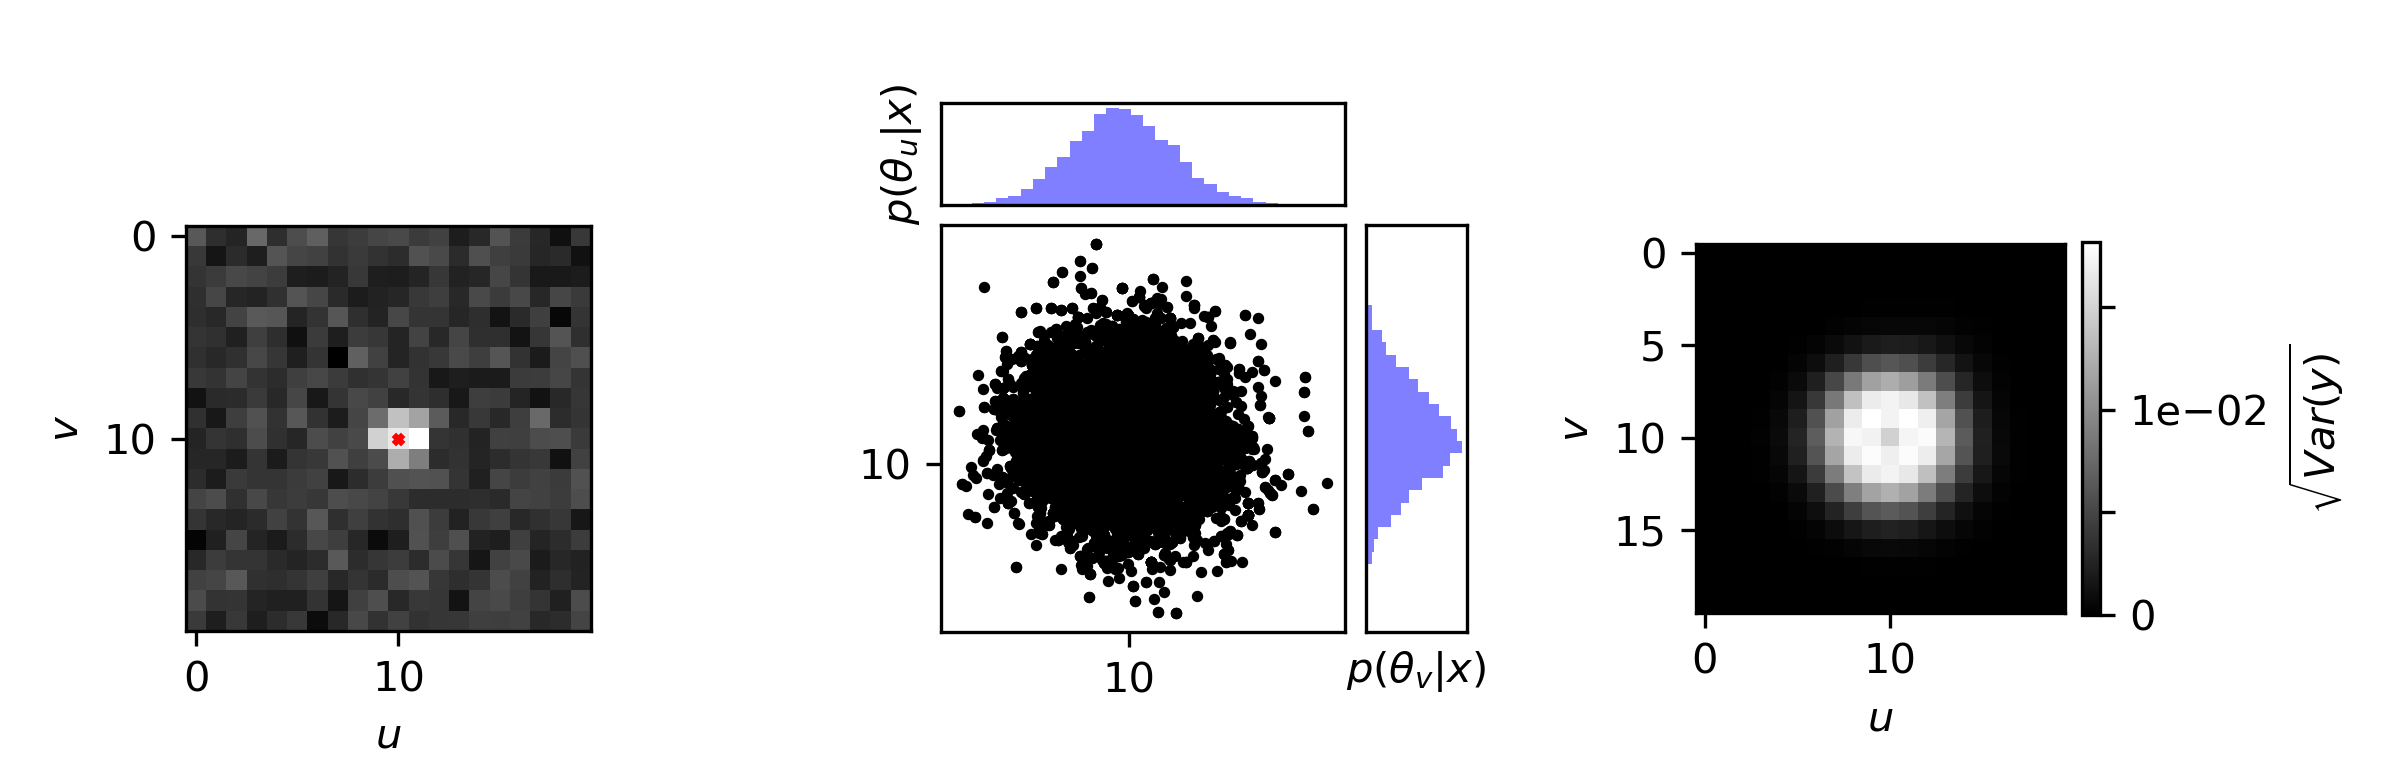
\includegraphics[scale=0.7]{/Users/cwseitz/git/cwseitz.github.io/docs/phd/ddpm/ddpm/media/MCMC.png}
\caption{Estimation of the marginal variances $\sqrt{\mathrm{Var}(\bold{y}_k)}$ for an isolated fluorescent emitter. MCMC sampling is carried out using the low-resolution image (left) to estimate the posterior $p(\theta\lvert\bold{x})$ (middle) which is sampled $\theta\sim p(\theta\lvert\bold{x})$ and combined with (3) to estimate marginal variances (right)}
\end{figure}

Similar to the generative process on low resolution images $\bold{x}$, we generate KDEs $\bold{y}$ by repurposing the generative model (1) on an unsampled image without noise. In other words, we cast Gaussian KD estimation as a noiseless image generation process on the domain of $\bold{y}$. Under a fixed configuration of $N$ particles $\theta$, the value of an non-normalized KDE pixel $\bold{y}_{k}$ is given by

\begin{equation}
\bold{y}_{k}(\theta) = \sum_{n=1}^{N}\Delta E_{u}(u_{k},\theta_{u},\sigma_{\bold{y}}) \Delta E_{v}(v_{k},\theta_{v},\sigma_{\bold{y}})
\end{equation}

where the hyperparameter $\sigma_{\bold{y}}$ is a Gaussian kernel width. 

\section{Uncertainty-Aware Localization Microscopy by Variational Diffusion}

We now consider more realistic datasets $(\bold{x}_i,\bold{y}_{0,i},\hat{\bold{y}}_{i})_{i=1}^{N}$ of observed images $\bold{x}_i$ true KD images $\bold{y}_{0,i}$, and augmented low-resolution inputs $\hat{\bold{y}}_{i}=\phi(\bold{x}_{i})$, where $\phi$ is a CNN. Observations $\bold{x}_i$ are simulated under the convolution distribution (1) and KDEs are generated by (4).

\subsection{Problem Statement}

Kernel density estimates produced by the traditional deep architectures for localization microscopy produce strong results, but lack uncertainty quantification. Unfortunately, the posterior $p(\theta\lvert\bold{x})$ has no known analytical form and can be difficult to compute at test time, since (i) molecules cannot be easily resolved and therefore $\theta$ is of unknown dimension and (ii) $\theta$ can be high dimensional and efficient exploration of the parameter space is challenging. The central goal of this paper is to instead model a conditional distribution on the latent $\bold{y}$: $p(\bold{y}\lvert\bold{x})$, where $\bold{y}$ is of known dimensionality. We choose to model $p(\bold{y}\lvert\bold{x})$ with a diffusion model, given that the distribution $p(\bold{y}\lvert\bold{x})$ is expensive to compute, even if $p(\theta\lvert\bold{x})$ were known.

Recent advances in generative modeling, particularly diffusion models \parencite{SohlDickstein2015,Ho2020,Song2021} present a unique opportunity to integrate uncertainty awareness into the localization microscopy toolkit. However, sampling from diffusion models can be computationally expensive, given that generation amounts to solving a complex stochastic differential equation, effectively mapping a simple base distribution to the complex data distribution. The solution of such equations requires numerical integration with very small step sizes, resulting in thousands of neural network evaluations \parencite{Saharia2021,Vahdat2021}. For conditional generation tasks in high-risk applications, generation complexity is further exacerbated by the need for the highest level of detail in generated samples. Therefore, we propose that sampling is preceded by an augmentation network $\phi$, which in essence generates an initial estimate to guide the diffusion process. Reasoning for this choice in our application is two-fold:

\textbf{Synthesis Speed}. By training the augmentation network $\phi$ to obtain an approximate estimate of $\bold{y}_{0}$, we can reduce the number of iterations, since the diffusion model only needs to model the remaining mismatch, resulting in a less complex model from which sampling becomes easier. Speed is critical in SMLM applications, which can produce thousands of images in a single experiment.\\

\textbf{Sample Fidelity}. Since Langevin dynamics will often be initialized in low-density regions of the data distribution, inaccurate score estimation in these regions will negatively affect the sampling process. Moreover, mixing can be difficult because of the need of traversing low density regions to transition between modes of the distribution \parencite{Song2019}.

\subsection{Variational Diffusion}


\begin{figure}[t]
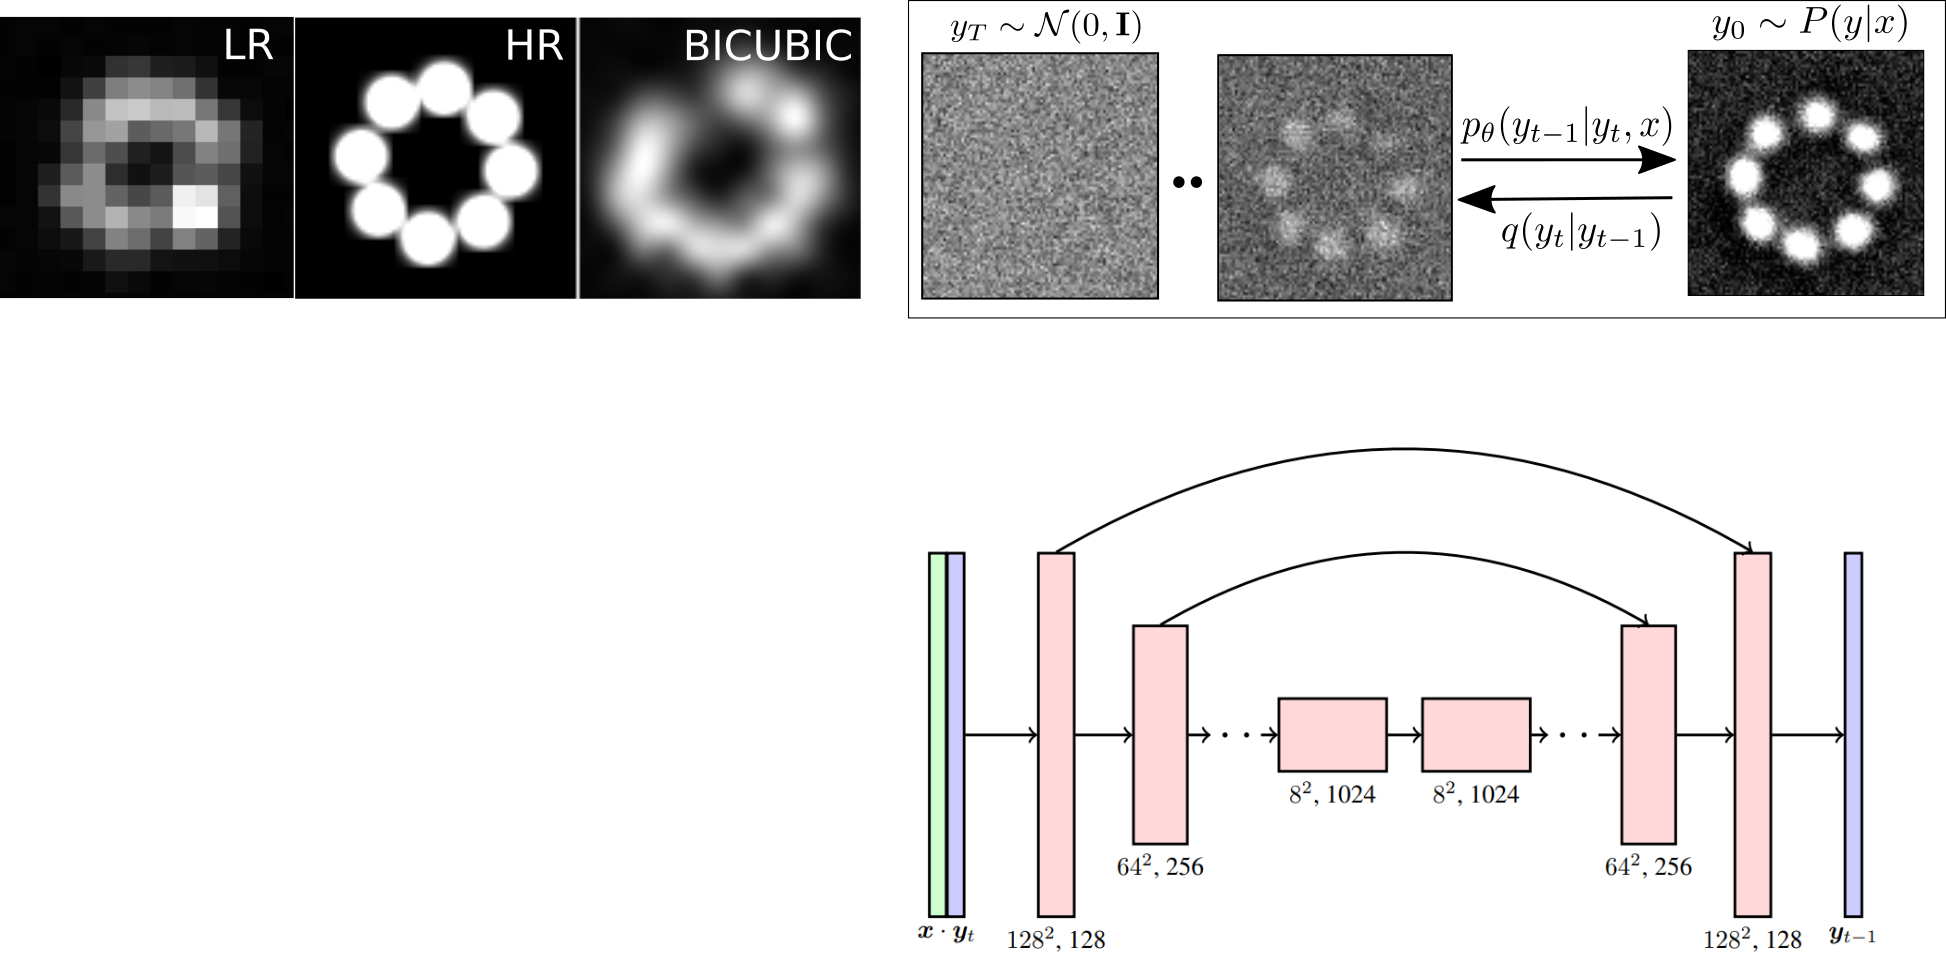
\includegraphics[scale=0.5]{/Users/cwseitz/git/cwseitz.github.io/docs/phd/ddpm/ddpm/media/Diffusion.png}
\end{figure}

Diffusion models \parencite{SohlDickstein2015,Ho2020,Song2021} are a class of generative models originally inspired by nonequilibrium statistical physics, which slowly destroy structure in a data distribution via a fixed Markov chain referred to as the \emph{forward process}. In the present context, we leverage the variational interpretation of this model class \parencite{Kingma2021,Kingma2023} to approximate the posterior $p(\bold{y}\lvert\bold{x})$. 

\textbf{Diffusion Model}. We use a forward process which gradually adds Gaussian noise to the latent $\bold{y}_0$ in discrete time, according to a variance schedule $\beta_{t}$:

\begin{equation}
q(\bold{y}_{T}\lvert\bold{y}_{0}) = \prod_{t=1}^{T}q(\bold{y}_{t}\lvert\bold{y}_{t-1}) \;\;\; q(\bold{y}_{t}\lvert\bold{y}_{t-1}) = \mathcal{N}\left(\sqrt{1-\beta_{t}}\bold{y}_{t-1},\beta_t I\right)
\end{equation}

An important property of the forward process is that it admits sampling $\bold{y}_t$ at an arbitrary timestep $t$ in closed form \parencite{Ho2020}. Using the notation $\alpha_t := 1 - \beta_t$ and $\gamma_t := \prod_{s=1}^{t} \alpha_s$, we have $q(\bold{y}_t\lvert\bold{y}_0) = \mathcal{N} \left(\sqrt{\gamma_{t}} \bold{y}_{0}, (1 - \gamma_t)I \right)$ or $\bold{y}_{t} = \sqrt{\gamma_{t}}\bold{y}_{0} + \sqrt{1-\gamma_{t}}\bold{\epsilon}$ for $\epsilon \sim \mathcal{N}(0,I)$. The signal to noise ratio (SNR) as defined in \parencite{Kingma2023}, at a time step $t$ reads $\mathrm{SNR}_t = \gamma_{t}/(1-\gamma_{t})$.

The usual procedure is then to learn a parametric representation of the \emph{reverse process}, and therefore generate samples of the latent $\bold{y}_{0}$ from  $p(\bold{y}_{0}\lvert\bold{x})$. Formally, $p_{\psi}(\bold{y}_{0}\lvert\bold{x}) = \int p_{\psi}(\bold{y}_{0:T}\lvert\bold{x})d\bold{y}_{1:T}$ where $\bold{y}_{t}$ is a latent representation with the same dimensionality of the data and $p_{\psi}(\bold{y}_{0:T}\lvert\bold{x})$ is a Markov process, starting from a noise sample $p_{\psi}(\bold{y}_{T}) = \mathcal{N}(0,I)$. Writing this Markov process gives

\begin{equation}
p_{\psi}(\bold{y}_{0:T}\lvert\bold{x}) = p_{\psi}(\bold{y}_{T})\prod_{t=1}^{T} p_{\psi}(\bold{y}_{t-1}\lvert\bold{y}_{t},\bold{x}) \;\;\; p_{\psi}(\bold{y}_{t-1}\lvert\bold{y}_{t},\bold{x}) = \mathcal{N}\left(\mu_{\psi}(\bold{y}_{t},\gamma_{t}),\beta_{t}I\right)
\end{equation}

where we reuse the variance schedule of the forward process \parencite{Ho2020}. From (5) it can be seen that the learnable parameter in the reverse process is the expectation of the transition $\mu_{\psi}$ where $\psi$ is a neural network. 

Learning the reverse process can be approached by either regressing noise $\bold{\epsilon}$ from the forward process, or the true latent $\bold{y}_{0}$, as there is a deterministic relationship between them. We adopt the former for consistency with other work, and define $\psi$ as a neural denoising function which regresses the noise $\bold{\epsilon}$ from a noisy $\bold{y}_{t}$. A relation between the noise estimate $\epsilon_{\psi}$ and $\mu_{\psi}$ is given in the Appendix, which gives an intuition for sampling. The proposed sampling scheme is depicted in (Figure 3). 

\textbf{Variational Objective}. Following \parencite{Kingma2021}, we interpret the reverse process as a hierarchical generative model that samples a sequence of latents $\bold{y}_{t}$, with time running backward. Training of the model is achieved through the variational bound

\begin{align}
-\log p(\bold{y}_{0}) &\leq -\mathbb{E}_{q(\bold{y}_{1:T}\lvert\bold{y}_{0})} \log \left(\frac{p_{\psi}(\bold{y}_{1:T},\bold{y}_{0})}{q(\bold{y}_{1:T}\lvert\bold{y}_{0})}\right) \\
&=  D_{KL}(q(\bold{y}_{T}\lvert\bold{y}_{0}) \lvert\lvert p(\bold{y}_{T})) + \mathbb{E}_{q(\bold{y}_{1}\lvert\bold{y}_{0})} \log p(\bold{y}_{0}\lvert\bold{y}_{1}) + \mathcal{L}_{\psi}
\end{align}

where we have omitted conditioning on the low-resolution $\bold{x}$ to simplify the notation. Note that, this is similar to a hierarchical VAE, but in a diffusion model $q(\bold{y}_{1:T}\lvert\bold{y}_{0})$ is fixed by the forward process rather than learned. The so-called diffusion loss $\mathcal{L}_{\psi}$ is shown in Appendix A, and is the term of interest as the first two terms do not contribute meaningfully to the loss \parencite{Ho2020}. Furthermore, it has become standard to use simplified forms of $\mathcal{L}_{\psi}$, such as a noise estimation loss, as this has shown superior performance. Importantly, $\mathcal{L}_{\psi}$ is simply a reweighted variant of a family of diffusion objectives \parencite{Kingma2021,Kingma2023}. We use the following Monte Carlo estimate of $\mathcal{L}_{\psi}$, which demonstrates that the variational bound can be written in terms of the common noise-estimation loss


\begin{equation}
\mathcal{L}_{\psi} = \mathbb{E}_{\epsilon\sim \mathcal{N}(0,I),t\sim U(1,T)}\left[\left(\frac{\mathrm{SNR}_{t-1}}{{\mathrm{SNR}_{t}}}-1\right)\lvert\lvert \bold{\epsilon}-\bold{\epsilon}_{\psi}\lvert\lvert_{2}^{2}\right]
\end{equation}

A full derivation of this objective is outlined in the Appendix. Note that $\mathrm{SNR}_{t}$ is monotonically decreasing with $t$, and thus $\frac{\mathrm{SNR}_{t-1}}{{\mathrm{SNR}_{t}}} = \frac{\gamma_{t-1}}{\gamma_{t}}\frac{1-\gamma_{t}}{1-\gamma_{t-1}} \geq 1$, ensuring $\mathcal{L}_{\psi}\geq 0$. In this paper, we choose to use a uniformly weighted loss and leave the exploration of the weighted loss to future work.

\section{Experiments}

All training data consits of low-resolution $20\times 20$ images, setting $\sigma_{\bold{x}}=0.92$ in units of low-resolution pixels, for consistency with common experimental conditions with a 60x magnification objective lens and numerical aperture (NA) of 1.4. We multiply $\omega_{k}$ by a constant $i_{0}=200$ for experiments for consistency with typical fluorophore emission rates. All KDEs have dimension $80\times 80$, are scaled between $[0,1]$, and are generated using $\sigma_{\bold{y}}=3.0$ pixels in the upsampled image. For a typical CMOS camera, this results in KDE pixels with lateral dimension of $\approx 27\mathrm{nm}$. Initial coordinates $\theta$ were drawn uniformly over a two-dimensional disc with a radius of 7 low-resolution pixels.


\begin{figure}
\centering
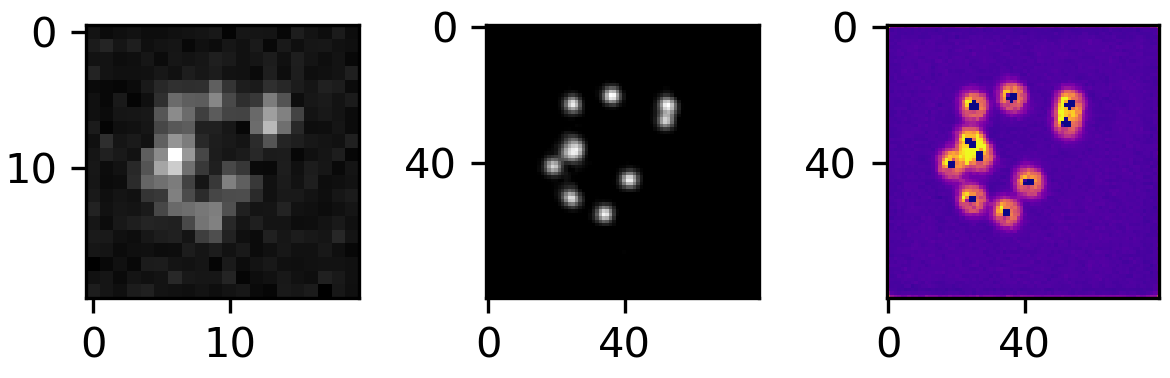
\includegraphics[scale=1.1]{/Users/cwseitz/git/cwseitz.github.io/docs/phd/ddpm/ddpm/media/Bayes.png}
\caption{Non cherry-picked estimation of marginal variances. A low-resolution image $\bold{x}$ (left column) is transformed by $\phi$ to produce a KDE estimate $\hat{\bold{y}}$ (middle column) and a DDPM $\psi$ computes a map of marginal variances (right column)}
\end{figure}

\textbf{Localization RMSE}. In order to verify the initial predictions made by the augmentation model $\phi$, we simulated a dataset $(\bold{x}_i,\bold{y}_{0,i},\hat{\bold{y}}_{i})_{i=1}^{N}$ with $N=1000$. Objects in the KDE $\hat{\bold{y}}_{i}$  are detected using the Laplacian of Gaussian (LoG) detection algorithm \parencite{Kong2013}, which permits more direct comparison of model predictions to the Cramer-Rao lower bound on localization error, compared to other image similarity measures. Localization is carried out from scale-space maxima directly in LoG, as opposed to fitting a model function to KDEs. A particular LoG localization in the KDE is paired to the nearest ground truth localization and is unpaired if a localization is not within 5 KDE pixels of any ground truth localization. In addition to localization error, we measure a precision $\mathrm{P = TP/(TP + FP)} = 1.0$ and recall $\mathrm{R = TP/(TP + FN)} = 0.85$, where $\mathrm{TP}$ denotes true positive localizations, $\mathrm{FP}$ denotes false positive localizations, and $\mathrm{FN}$ denotes false negative localizations.


\textbf{Variational Diffusion}. We set $T = 100$ for all experiments and treat forward process variances $\beta_{t}$ as hyperparameters, with a linear schedule from $\beta_{0}=10^{-4}$ to $\beta_{T}=10^{-2}$.
These constants were chosen to be small relative to ground truth KDEs, which are scaled to $[-1,1]$, ensuring that forward process distribution $\bold{y}_{T}\sim q(\bold{y}_{T}\lvert\bold{y}_{0})$ approximately matches the reverse process $\bold{y}_T\sim \mathcal{N}(0, I)$ at $t=T$. Example KD estimates from low-resolution images and the marginal variances obtained from sampling $N=100$ samples from $p_{\psi}(\bold{y}_{0}\lvert\bold{x})$ are shown in (Figure 4). 


\section{Conclusion}

We proposed a variational diffusion model for uncertainty-aware localization microscopy. Our approach builds on recent advancements in conditional diffusion models, to model the posterior distribution on high-resolution KD estimates from low-resolution inputs. This tractable posterior distribution is constructed by first augmenting low resolution inputs to a KD estimate using the DeepSTORM architecture with minor modifications \parencite{Nehme2020}. Conditioning a diffusion model on this initial estimate permits sampling with relatively fewer samples than most existing diffusion models in similar applications, thereby making computation of marginal variances possible. Our approach made three core contributions: (i) we derived a relationship between the posterior on kernel density estimates with the posterior on molecular locations, and (ii) we demonstrated that a diffusion model can model a distribution on KDEs with qualitatively similar marginal variances expected from predictions made using MCMC. By using a recently discovered relationship of the variational lower bound to a traditional noise-estimation objective, we can confidently approximate the true posterior.

\section{Broader Impact}

The development of a method for uncertainty estimation in super-resolution imaging, as proposed here, holds implications beyond its immediate application in SMLM. By leveraging diffusion models for uncertainty estimation, this approach not only enhances the reliability of super-resolution image reconstructions but also extends its utility to a diverse array of domains. The incorporation of a guided diffusion process facilitates efficient reconstruction while maintaining intepretation of the underlying uncertainty. Importantly, the principles underlying this method resonate across various fields, suggesting its potential applicability in domains beyond microscopy. For instance, the extension of similar techniques to general image processing tasks highlights the potential to address uncertainty in a wide range of applications in bioimaging or medical imaging. Moreover, the utilization of diffusion models for uncertainty estimation aligns with a broader trend in leveraging probabilistic frameworks for enhancing deep learning applications, with implications extending to fields such as natural language processing, computer vision, and autonomous systems. By bridging these interdisciplinary boundaries, this method not only addresses a critical need in localization microscopy but also contributes to the advancement of uncertainty-aware deep learning methodologies.


\section{Appendix}

\begin{figure}[t]
\centering
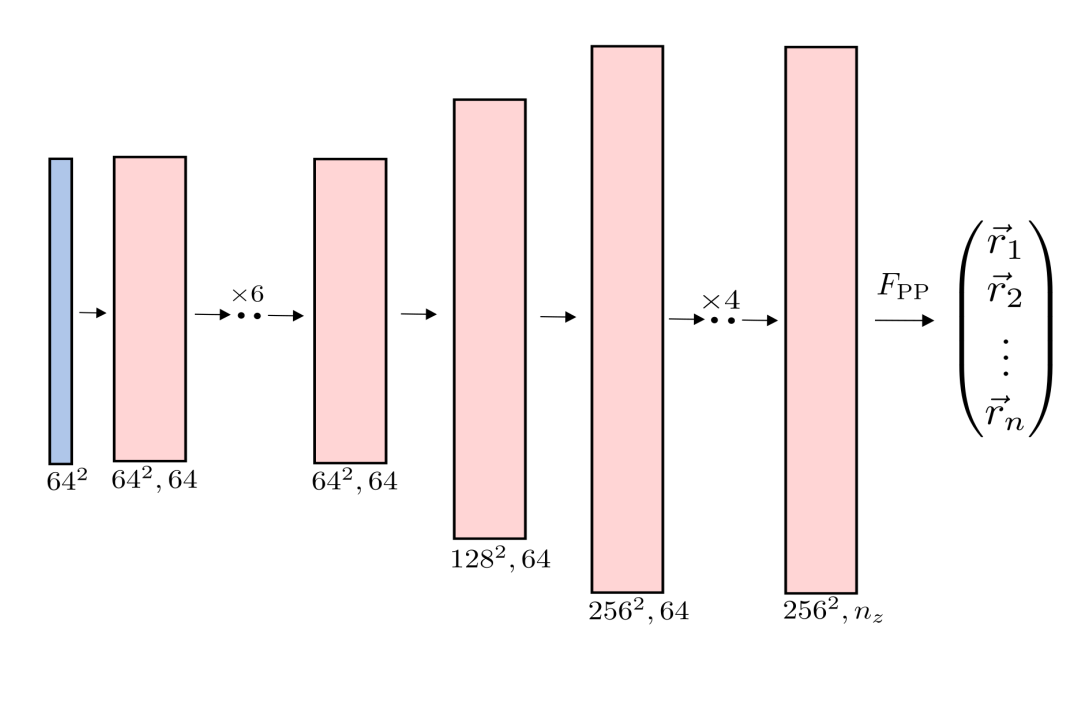
\includegraphics[scale=0.4]{/Users/cwseitz/git/cwseitz.github.io/docs/phd/dissertation/dissertation/media/DeepSTORM.png}
\end{figure}
\begin{figure}[t]
\centering
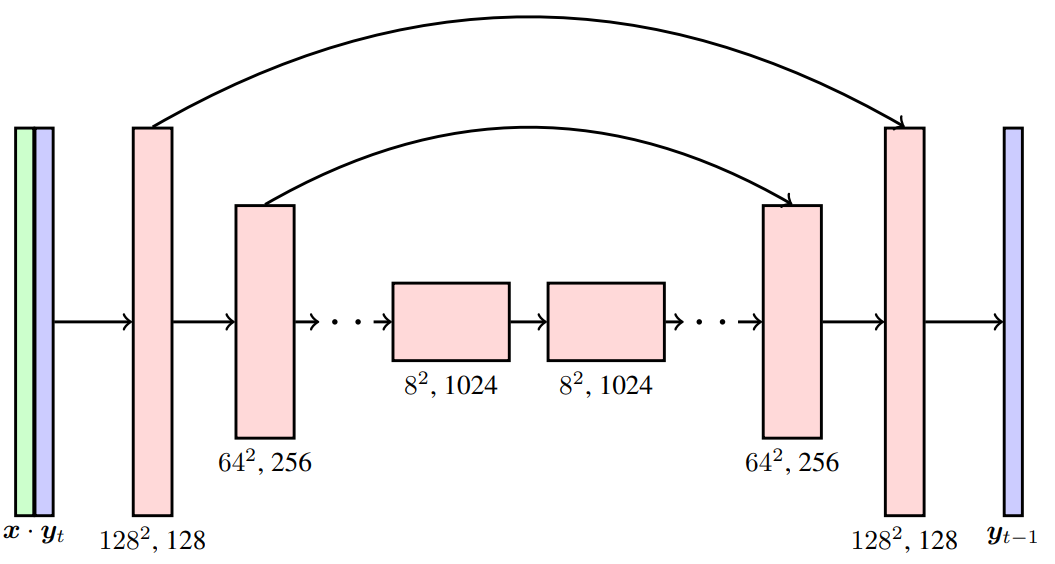
\includegraphics[scale=0.4]{/Users/cwseitz/git/cwseitz.github.io/docs/phd/dissertation/dissertation/media/DiffusionArch.png}
\end{figure}

\subsection{Sampling}

Sampling from the reverse process $p_{\psi}(\bold{y}_{t-1}\lvert\bold{y}_{t},\bold{x})$ is achieved by estimation of the noise $\epsilon_{\psi}$ from $\bold{y}_{t}$ by the denoising model $\psi$, and therefore estimation of $\bold{y}_{0}$

\begin{equation}
\hat{\bold{y}}_{0} = \frac{1}{\sqrt{\gamma_{t}}}(\bold{y}_{t} - \sqrt{1-\gamma_{t}}\epsilon_{\psi})
\end{equation}

followed by sampling from the forward process $\bold{y}_{t-1} \sim q(\bold{y}_{t-1}\lvert\hat{\bold{y}}_{0}) = \mathcal{N}(\sqrt{\gamma_{t-1}},(1-\gamma_{t-1})I)$. 


\subsection{Derivation of the variational bound}

We now derive the so-called diffusion loss $\mathcal{L}_{\psi}$, written in (8) in the main text. Similar derivations can be found in \parencite{Kingma2021,Ribeiro2024}, and we include it here only for completeness

\begin{align*}
-\log p(\bold{y}_{0}) &\leq - \mathbb{E}_{q(\bold{y}_{1:T}\lvert\bold{y}_{0})} \log \frac{p(\bold{y}_{0:T})}{q(\bold{y}_{1:T}\lvert\bold{y}_{0})}\\
&= -\mathbb{E}_{q(\bold{y}_{1:T}\lvert\bold{y}_{0})} \log \frac{p(\bold{y}_{T})p(\bold{y}_0\lvert\bold{y}_1) \prod_{t=2}^{T}p(\bold{y}_{t-1}\lvert\bold{y}_t)}{q(\bold{y}_T\lvert\bold{y}_0)\prod_{t=2}^{T}q(\bold{y}_{t-1}\lvert\bold{y}_t,\bold{y}_0)}\\
&= -\mathbb{E}_{q(\bold{y}_{1:T}\lvert\bold{y}_{0})} \left[ p(\bold{y}_0\lvert\bold{y}_1) + \log \frac{p(\bold{y}_{T})}{q(\bold{y}_T\lvert\bold{y}_0)} + \sum_{t=2}^{T} \log \frac{p(\bold{y}_{t-1}\lvert\bold{y}_t)}{q(\bold{y}_{t-1}\lvert\bold{y}_t,\bold{y}_0)}\right]\\
&= -\mathbb{E}_{q(\bold{y}_{1:T}\lvert\bold{y}_{0})} \left[ p(\bold{y}_0\lvert\bold{y}_1)\right] + D_{KL}\left(q(\bold{y}_T\lvert\bold{y}_0) \lvert\lvert p(\bold{y}_{T})\right) \\
&+ \sum_{t=2}^{T} \mathbb{E}_{q(\bold{y}_{t}\lvert\bold{y}_{0})} D_{KL}\left(q(\bold{y}_{t-1}\lvert\bold{y}_t,\bold{y}_0)\lvert\lvert p(\bold{y}_{t-1}\lvert\bold{y}_t) \right)
\end{align*}

As before, we omit conditioning on $\bold{x}$ to simplify the notation. The first term is typically ignored, as it does not contribute meaningfully to the loss \parencite{Ribeiro2024}. Furthermore, the second term is approximately zero by construction. Therefore we are left with the last term, called the diffusion loss $\mathcal{L}_{\psi}$. The KL-divergence of $q$ and $p$ is between two Gaussians with identical variances $\sigma^{2} = \frac{(1-\gamma_{t-1})(1-\alpha_{t})}{1-\gamma_{t}}$, and expectations

\begin{align*}
\mu = \frac{\sqrt{\gamma_{t-1}}(1-\alpha_{t})}{1-\gamma_{t}}\bold{y}_{0}+ \frac{\sqrt{\alpha_{t}}(1-\gamma_{t-1})}{{1-\gamma_{t}}}\bold{y}_{t} \quad \mu_{\psi} = \frac{\sqrt{\gamma_{t-1}}(1-\alpha_{t})}{1-\gamma_{t}}\hat{\bold{y}}_{0}+ \frac{\sqrt{\alpha_{t}}(1-\gamma_{t-1})}{{1-\gamma_{t}}}\bold{y}_{t}
\end{align*}

for a fixed noise schedule \parencite{Saharia2021}. Therefore, we have

\begin{align*}
D_{KL}\left(q(\bold{y}_{t-1}\lvert\bold{y}_t,\bold{y}_0)\lvert\lvert p(\bold{y}_{t-1}\lvert\bold{y}_t) \right) &= \frac{1}{2\sigma^{2}} \lvert\lvert \mu - \mu_{\psi} \lvert\lvert_{2}^{2} \\
&= \frac{1}{2}\frac{\gamma_{t-1}(1-\alpha_{t})}{(1-\gamma_{t-1})(1-\gamma_{t})}\lvert\lvert \bold{y}_{0} - \hat{\bold{y}}_{0} \lvert\lvert_{2}^{2}\\
&= \frac{1}{2}\frac{\gamma_{t-1}((1-\gamma_{t})-\alpha_{t}(1-\gamma_{t-1}))}{(1-\gamma_{t-1})(1-\gamma_{t})}\lvert\lvert \bold{y}_{0} - \hat{\bold{y}}_{0} \lvert\lvert_{2}^{2}\\
&= \frac{1}{2}\frac{\gamma_{t-1}((1-\gamma_{t})-\frac{\gamma_{t}}{\gamma_{t-1}}(1-\gamma_{t-1}))}{(1-\gamma_{t-1})(1-\gamma_{t})}\lvert\lvert \bold{y}_{0} - \hat{\bold{y}}_{0} \lvert\lvert_{2}^{2}\\
&= \frac{1}{2}\left(\frac{\gamma_{t-1}}{1-\gamma_{t-1}}-\frac{\gamma_{t}}{1-\gamma_{t}}\right)\lvert\lvert \bold{y}_{0} - \hat{\bold{y}}_{0} \lvert\lvert_{2}^{2}\\
&= \frac{1}{2}\left(\mathrm{SNR}_{t-1}-\mathrm{SNR}_{t}\right)\lvert\lvert \bold{y}_{0} - \hat{\bold{y}}_{0} \lvert\lvert_{2}^{2}
\end{align*}

Reparameterizing the loss in terms of the noise, using $\lvert\lvert \bold{y}_{0} - \hat{\bold{y}}_{0} \lvert\lvert_{2}^{2} = \frac{1-\gamma_{t}}{\gamma_{t}}\lvert\lvert \bold{\epsilon}_{0} - \epsilon_{\psi} \lvert\lvert_{2}^{2}$ \parencite{Ribeiro2024}, we arrive at 

\begin{equation*}
\mathcal{L}_{\psi} = \frac{1}{2}\sum_{t=2}^{T} \mathbb{E}_{q(\bold{y}_{t}\lvert\bold{y}_{0})}\left(\frac{\mathrm{SNR}_{t-1}}{{\mathrm{SNR}_{t}}}-1\right)\lvert\lvert \bold{\epsilon}-\bold{\epsilon}_{\psi}\lvert\lvert_{2}^{2}
\end{equation*}

Using a Monte Carlo estimate of $\mathcal{L}_{\psi}$ \parencite{Kingma2023} which optimizes random terms of the summation to avoid calculating all terms simultaneously, we arrive at the objective written in the main text (8)

\begin{equation*}
\mathcal{L}_{\psi} = \mathbb{E}_{\epsilon\sim \mathcal{N}(0,I),t\sim U(1,T)}\left[\left(\frac{\mathrm{SNR}_{t-1}}{{\mathrm{SNR}_{t}}}-1\right)\lvert\lvert \bold{\epsilon}-\bold{\epsilon}_{\psi}\lvert\lvert_{2}^{2}\right]
\end{equation*}

\subsection{Metropolis-Hastings MCMC}

To obtain numerical estimates of $p(\theta\lvert\bold{x})\propto p(\bold{x}\lvert\theta)p(\theta)$ and therefore $p(\bold{y}\lvert\bold{x})$, for the isolated fluorescent molecule as shown in (Figure 2), we used Metropolis-Hastings Markov Chain Monte Carlo (MCMC) to estimate the posterior on coordinates. Under the Poisson approximation in (1), the model negative log-likelihood is

\begin{equation}
\ell(\bold{x}\lvert\theta) = -\log \prod_{k} \frac{e^{-\left(\omega_{k}'\right)}\left(\omega_{k}'\right)^{n_{k}}}{n_{k}!} = \sum_{k}  \log n_{k}! + \omega_{k}' - n_{k}\log\left(\omega_{k}'\right)
\end{equation}

where $n_{k}$ is the observed number events at a pixel. MCMC is asymptotically exact, which is not guaranteed by variational methods which may rely on a Laplace approximation around the MLE. We choose a uniform prior $p(\theta)$, and Metropolis-Hastings is run for $10^4$ iterations, the first $10^{3}$ iterations are discarded as burn-in. A proposal $\theta' = \theta + \Delta\theta$ was generated with $\Delta\theta \sim \mathcal{N}(0,\sigma^{2}I)$ where $\sigma^{2}=0.05$. The acceptance probability is

\begin{equation*}
\alpha = e^{\beta(\ell(\theta)-\ell(\theta'))}
\end{equation*}

We choose $\beta=0.2$ to achieve a target acceptance rate of $0.5$.

\subsection{Cramer-Rao Lower Bound}

Reliable inference of $\theta$ from $\bold{x}$ in general requires performance metrics for model selection. We use the Fisher information as an information theoretic criteria to assess the quality of the data augmentation model $\phi$ tested here, with respect to the root mean squared error (RMSE) of our predictions of $\theta$ \parencite{Chao2016}. The Poisson log-likelihood $\ell(\bold{x}\lvert\theta)$ is also convenient for computing the Fisher information matrix \parencite{Smith2010} and thus the Cramer-Rao lower bound, which bounds the variance of a statistical estimator of $\theta$, from below i.e., $\mathrm{var}(\hat{\theta}) \geq I^{-1}(\theta)$. The Fisher information is straightforward to compute under the Poisson log-likelihood in (1). In general, the Fisher information is given by the expression

\begin{equation}
I_{ij}(\theta) = \underset{\theta}{\mathbb{E}}\left(\frac{\partial \ell}{\partial\theta_{i}}\frac{\partial\ell}{\partial\theta_{j}}\right) 
\end{equation}

For an arbitrary parameter, we find that, for a Poisson log-likelihood $\ell$

\begin{align*}
\frac{\partial \ell}{\partial \theta_{i}} &= \frac{\partial}{\partial \theta_{i}} \sum_{k}  \log n_{k}! + \omega_{k}' - n_{k}\log\left(\omega_{k}'\right)\\
&= \sum_{k} \frac{\partial \omega_{k}'}{\partial\theta_{i}} \left(\frac{\omega_{k}'-n_{k}}{\omega_{k}'}\right)
\end{align*}

Using this result, we can compute the Fisher information matrix $I(\theta)$

\begin{equation*}
I_{ij}(\theta) = \underset{\theta}{\mathbb{E}}\left(\sum_{k}\frac{\partial \omega_{k}'}{\partial\theta_{i}}\frac{\partial \omega_{k}'}{\partial\theta_{j}} \left(\frac{\omega_{k}'-n_{k}}{\omega_{k}'}\right)^{2}\right) = \sum_{k}\frac{1}{\omega_{k}'}\frac{\partial \omega_{k}'}{\partial\theta_{i}}\frac{\partial \omega_{k}'}{\partial\theta_{j}}
\end{equation*}

A fundamental lower bound on the variance in our estimates of $\theta$ then is found from its inverse: $\mathrm{CRLB} = I^{-1}(\theta)$. This result is used to show in (Figure 5), that the data augmentation model $\phi$ efficiently estimates molecular coordinates under the experimental conditions tested here. 


\begin{figure}[t]
\centering
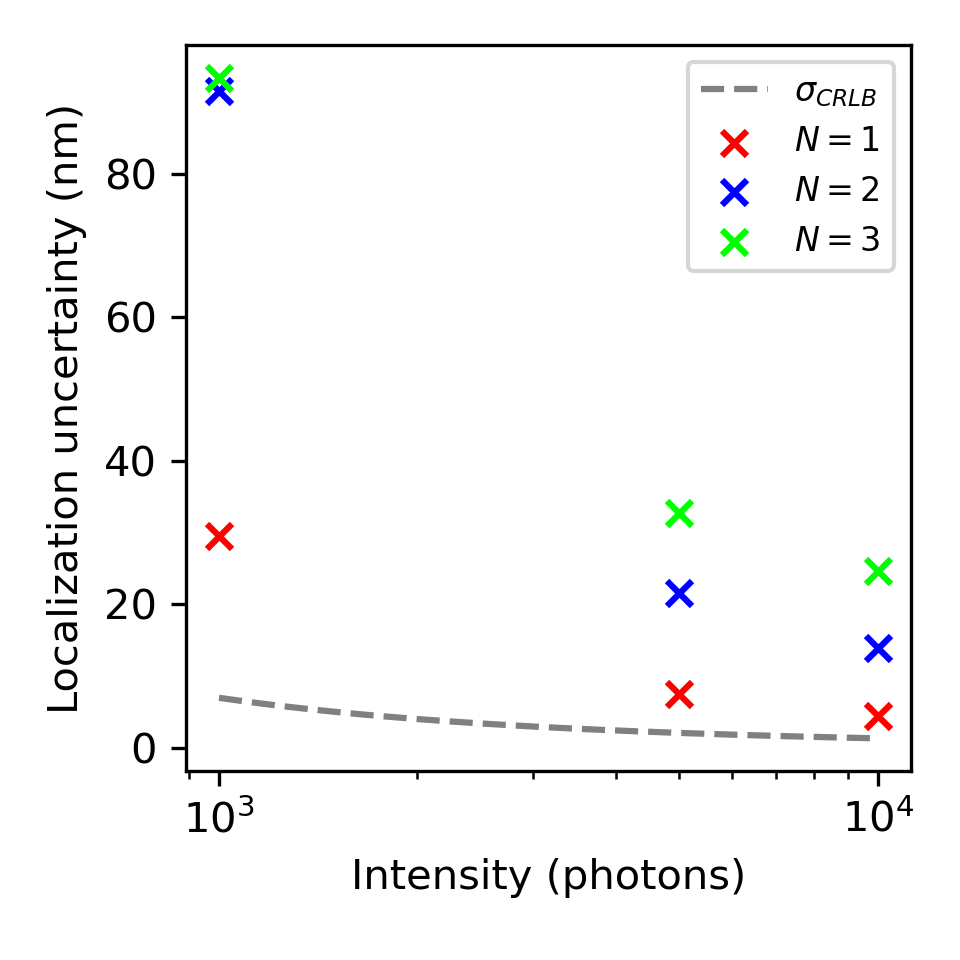
\includegraphics[scale=0.7]{/Users/cwseitz/git/cwseitz.github.io/docs/phd/ddpm/ddpm/media/Errors.png}
\caption{Localization errors of the trained model $\phi$. The Cramer-Rao lower bound is shown in red, computing by taking the diagonal elements of $I^{-1}(\theta)$.}
\end{figure}


\subsection{Neural Networks $\psi,\phi$}

\textbf{DeepSTORM CNN $\phi$}. The DeepSTORM CNN, for 3D localization, can be viewed as a deep kernel density estimator, reconstructing kernel density estimates $\bold{y}$ from low-resolution inputs $\bold{x}$. We utilize a simplified form of the original architecture \parencite{Nehme2020} for 2D localization, which we denote $\phi$ in this paper, which consists of three main modules: a multi-scale context aggregation module, an upsampling module, and a prediction module. For context aggregation, the architecture utilizes dilated convolutions to increase the receptive field of each layer. The upsampling module is then composed of two consecutive 2x resize-convolutions, computed by nearest-neighbor interpolation, to increase the lateral resolution by a factor of 4. Additional details regarding this architecture can be found in the original paper \cite{Nehme2020}. The terminal prediction module contains three additional convolutional blocks for refinement of the upsampled image, followed by an element-wise HardTanh. The architecture is trained using the objective $\mathcal{L}_{\phi} = \frac{1}{N}\sum_{n=1}^{N} (\bold{y}_{0,n}-\bold{\hat{y}}_{n})^{2}$. 

\textbf{DDPM $\psi$}. To represent the reverse process, we used a DDPM architecture originally proposed in \parencite{Saharia2021}. We chose the U-Net backbone to have channel multipliers $[1,2,4,8,8]$ in the downsampling and upsampling paths of the architecture. In this architecture, parameters are shared across time, which is specified to the network using the Transformer sinusoidal position embedding, and uses self-attention at the $16 \times 16$ feature map resolution. To condition the model on the input $\bold{\hat{y}}$, we concatenate the $\bold{\hat{y}}$ estimated by DeepSTORM along the channel dimension, which are scaled to $[0,1]$, with $\bold{y}_T\sim \mathcal{N}(0, I)$. Others have experimented with more sophisticated methods of conditioning, but found that the simple concatenation yielded similar generation quality \parencite{Saharia2021}. 


